\chapter{Présentation du cadre du projet} 
 
 \addcontentsline{toc}{chapter}{Chapitre 1 : Présentation du cadre du projet}
\markboth{Chapitre 1 : Présentation du cadre du projet}{}
\phantomsection % Crée un point d'ancrage pour les hyperliens dans le document
\addcontentsline{toc}{section}{Introduction} % Ajoute "Introduction" dans la table des matières

\section*{Introduction} % Affiche le titre sans numérotation
Dans ce présent chapitre nous avons présenté l’organisme d’accueil, et ses principales activités. Nous avons aussi évoqué la problématique, la solution, l’objectif à atteindre et la planification de notre projet.
\renewcommand{\thesection}{\Roman{section}.} % I, II, ...
\renewcommand{\thesubsection}{\arabic{subsection}.} % 1, 2, ...
\renewcommand{\thesubsubsection}{\thesubsection\arabic{subsubsection}} % I.1, I.2 ...

% Ce qui suit force l’affichage du numéro des subsubsections
\setcounter{secnumdepth}{3} 
\section{Présentation de l'organisme d'accueil}
\subsection{Situation géographique:}
\begin{itemize}
    \item Entreprise : OMINET SARL 
    \item Adresse : Centre Urbain Nord, Tunis. 
    \item Horaires : De 8h à 12h et de 14h à 17h.
\end{itemize}

OMINET SARL, héritière de Coccinet fondée en 2014, est une agence offshore spécialisée dans la création de sites Internet et les solutions digitales sur mesure. Grâce à une équipe d'experts expérimentés, l’entreprise accompagne ses clients dans le développement de leur présence en ligne.

Classée comme une PME (Petite et Moyenne Entreprise), OMINET SARL dispose de plusieurs départements, dont un département commercial et un département technique. L'équipe, composée de [insérer nombre de collaborateurs et stagiaires], est dirigée par un gestionnaire principal.

Depuis sa création, OMINET SARL s'engage à offrir des solutions adaptées aux besoins de ses clients, avec pour objectif principal de maximiser leur satisfaction. L’entreprise met tout en œuvre pour développer des outils digitaux innovants, permettant à ses clients de booster leur performance et d’atteindre leurs objectifs stratégiques.


\subsection{Historique de Coccinet:}
Coccinet est une société à responsabilité limitée (SARL), immatriculée sous le SIREN 479824914, et en activité depuis 18 ans. Basée à Paris (75011), elle se spécialise dans le secteur de la programmation informatique.

Avec un effectif de 6 à 9 salariés, l’entreprise a réalisé un chiffre d'affaires de 200 300 € en 2012, marquant une augmentation notable de 43,64 du total du bilan entre 2011 et 2012.

Depuis sa création, Coccinet a vu plusieurs évolutions importantes, notamment l’enregistrement de différents établissements et mandataires. Le dernier événement notable de l’entreprise remonte au 28 décembre 2021.

Actuellement, l’entreprise est dirigée par Maxence Caillaud, son gérant, qui continue de piloter Coccinet dans ses projets et son développement dans le domaine des solutions informatiques.

\subsection{Organigramme}
L'organigramme de l'OMINET est représenté dans la figure ci-dessous :

\begin{figure}[H]
  \centering
  \begin{minipage}{0.45\textwidth}
    \centering
    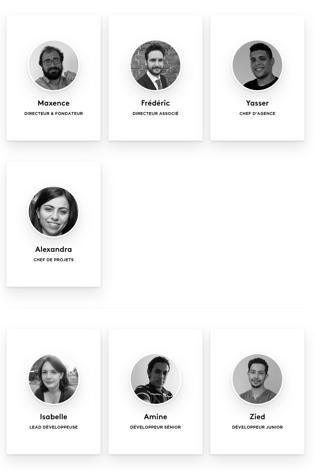
\includegraphics[width=\linewidth]{projet/images/diagramme de sequance/images/omminet.png}
  \end{minipage}
  \hfill
  \begin{minipage}{0.45\textwidth}
    \centering
    
\includegraphics[width=\linewidth]{projet/images/diagramme de sequance/images/omminet1.png}
  \end{minipage}
  \caption{L’organigramme de l’OMINET}
\end{figure}
\section{Etude préalable }
\subsection{Critique de l’existant}
En regardant de plus près, voici ce qui pose problème avec ces méthodes :
\begin{itemize}[label=$\rightarrow$]
    \item \textbf{Perte de temps et d’énergie :} \\
    Les organisateurs et participants perdent beaucoup de temps à gérer ou chercher des informations. Et même avec les recherches, les résultats ne sont pas toujours fiables.
    \item \textbf{Problème des places limitées :} \\
    Quand un événement est complet, il n’y a pas de moyen simple pour gérer les gens en liste d’attente. Cela crée de la frustration, car des participants motivés passent à côté.
    \item \textbf{Mauvaise communication :} \\
    Sans système intégré, les annonces ou rappels ne sont pas toujours bien diffusés, ce qui complique la tâche pour tout le monde.
    \item \textbf{Manque d’analyse :} \\
    Il est difficile pour les organisateurs d’avoir une vue claire des statistiques, comme le nombre d’inscrits ou les retours des participants.
    \item \textbf{Plateformes peu adaptées :} \\
    Certaines solutions existantes ne sont pas faites pour de petites structures, soit parce qu’elles sont trop chères, soit parce qu’elles ne correspondent pas aux besoins.
\end{itemize}

\subsection{Problématique:}
Actuellement, les associations, clubs et autres communautés en Tunisie utilisent des méthodes classiques ou des outils simples pour gérer leurs événements, mais ces solutions ne répondent pas toujours à leurs besoins. Voici ce qu’on remarque :
\begin{enumerate}
    \item \textbf{Méthodes traditionnelles :} \\
    Les organisateurs gèrent souvent leurs inscriptions avec des fichiers Excel ou des listes papier. C’est simple mais vite inefficace quand il y a beaucoup de participants.
    \item \textbf{Outils en ligne limités :} \\
    Il existe des plateformes pour créer et gérer des événements, mais elles ne permettent pas forcément de gérer les inscriptions correctement, surtout quand les places sont limitées.
    \item \textbf{Communication dispersée :} \\
    Pour informer les participants, on passe par WhatsApp, des e-mails, ou des publications sur Facebook. C’est compliqué et parfois les gens ratent l’information importante.
    \item \textbf{Peu de retours d’expérience :} \\
    Les outils actuels n’aident pas vraiment à analyser les événements (comme voir combien de personnes se sont inscrites ou ce qui a bien fonctionné).
    \item \textbf{Accessibilité :}  \\
    Certaines plateformes sont trop chères ou compliquées à utiliser pour les petites associations ou clubs.
\end{enumerate}
\subsection{Solution proposée}
Notre plateforme apporte des solutions modernes pour simplifier la gestion des événements et répondre aux besoins des organisateurs :
\begin{itemize}[label=$\star$]
  \item \textbf{Inscriptions faciles :} \\
  Une interface intuitive permet de gérer les inscriptions, les annulations, et les listes d’attente automatiquement.
  \item \textbf{Communication rapide :} \\
  Avec un système de messagerie intégré et des notifications push, les organisateurs peuvent rester connectés avec les participants en temps réel.
  \item \textbf{Suivi clair :} \\
  Un tableau de bord analytique fournit des statistiques sur les inscriptions et les retours des participants, aidant les organisateurs à mieux planifier.
  \item \textbf{Accessibilité pour tous :} \\
  Simple, abordable et adaptée même aux petites communautés, la plateforme est facile à prendre en main sans expertise technique.
  \item \textbf{Gestion des places limitées :} \\
  Les participants peuvent rejoindre une liste d’attente et être notifiés dès qu’une place est disponible.
\end{itemize}
\section {Méthodologie adaptées}
Dans cette section, nous examinons en détail les méthodes utilisées qui nous ont permis de progresser dans la réalisation de notre projet.
\subsection{Méthodologie de modélisation et de conception}
En utilise le méthodologie de modélisation et de conception  pour mieux comprendre les besoins et planifier techniquement le projet .

Le langage UML (Unified Modeling Language, ou langage de modélisation unifié) a été pensé pour être un langage de modélisation visuelle commun, et riche sémantiquement et syntaxiquement.Son objectif est de concevoir et mettre en place des systèmes logiciels complexes en termes de structure et de comportement. Les applications de l’UML dépassent le domaine du développement logiciel, en particulier pour les flux de processus dans le secteur industriel.\cite{ref1}
\subsection{Methodologie de gestion de projet }
Dans le domaine de developpement web , les projets informatiques deviennent de plus en plus complexes avec l’évolution rapide des technologies et des besoins , alors en va Développer une approche stratégique pour repondre au besoin du client car les anciennes méthodes de gestion rigides ne répondent plus à cette réalité . dans ce cas l’approche Agile s’est imposée comme une solution moderne et efficace.

La méthode agile est une méthode de gestion de projet. L’idée, lorsque l’on utilise cette approche, est d’apporter souplesse et performance à la gestion de projet. Centrée sur l’humain et la communication, elle permet aux clients de participer au développement d’un produit tout au long de l’avancement du projet.\cite{ref2} .
Dans ce maniére en utilise le méthode SCRUM pour ce projet 

Scrum C'est la méthode de travail la plus répandue pour la gestion des projets agile et divise le travail dans un équipe .

Scrum est une structure Agile qui facilite la collaboration au sein des équipes et les aide à réaliser des tâches à haute valeur ajoutée. Elle propose un schéma de valeurs, rôles et directives pour leur permettre de se concentrer sur chaque itération et de s’améliorer en continu.\cite{ref3}

\textbf{Principes fondamentaux : }\\
\textbf{•	Collaboration :   } Les équipes travaillent ensemble de manière collaborative. \\
\textbf{•	Itération } Le travail est divisé en sprints (généralement de 2 à 4 semaines). \\
\textbf{•	Adaptabilité }Les exigences peuvent évoluer en fonction des retours des utilisateurs.
\subsubsection{Rôles dans Scrum :}
Le methode scrum définit trois rôles principaux :

 \begin{itemize}
    \item[$\star$] \textbf{Product Owner : }traduit les besoins du client en tâches concrètes pour l’équipe, tout en s’assurant que les priorités sont claires et alignées avec les objectifs du projet. 
 \item[$\star$]\textbf{Scrum Master : }il accompagne l’équipe au quotidien en veillant à ce que le cadre Scrum soit respecté, tout en aidant chacun à avancer malgré les blocages éventuels.
 \item[$\star$]\textbf{Équipe de Développement : } qui transforme les idées en solutions concrètes, en collaborant activement pour livrer un produit fonctionnel et de qualité . 
\end{itemize}
\subsubsection{ Artefacts de Scrum :}
Les artefacts de scrum permet de  de gérer le travail .
 \begin{itemize}
\item[$\star$] \textbf{Product Backlog : } Il contient toutes les idées, fonctionnalités et améliorations à venir. Il se met à jour au fur et à mesure que le projet avance, afin de s’assurer que les priorités restent alignées avec les besoins réels du client.
\item[$\star$]\textbf{Sprint Backlog : } C’est la liste des tâches que l’équipe doit accomplir en fonction de ses capacités et des priorités du moment, choisies directement à partir du Product Backlog
\item[$\star$]\textbf{ Increment : }C'est un livrable qui doit être fonctionnel et prêt à être déployé, garantissant que chaque itération apporte une réelle valeur ajoutée au projet.
\end{itemize}
\subsubsection{Processus Scrum : }
Le Processus Scrum comporte plusieurs étapes.
 \begin{itemize}
    \item[$\star$] \textbf{ sprint meeting planning : } Est un moment où l'équipe trier les éléments du product backlog à réaliser durant le sprint.
et définies les tâches spécifiques  pour chaque élément sélectionné.
      \item[$\star$] \textbf{ Daily Scrum : }  faire une réunion quotidienne de 15 minutes pour cadrer l'équipe et chaque membre partage son travail et  présente les difficultés rencontrées.
       \item[$\star$] \textbf{Le sprint review : } le Product Owner invite l’équipe Scrum et les parties prenantes, et l’équipe presente ce qu’il  a fait.Les parties prenantes donnent leur avis, pour permet d'améliorer le produit et d’ajuster le backlog.
        \item[$\star$] \textbf{Sprint Rétrospective : } c'est la dernier réunions ,on discute sur ce qui a bien fonctionné et ce qui peut être amélioré .
\end{itemize}
\begin{figure}[H]
    \centering
    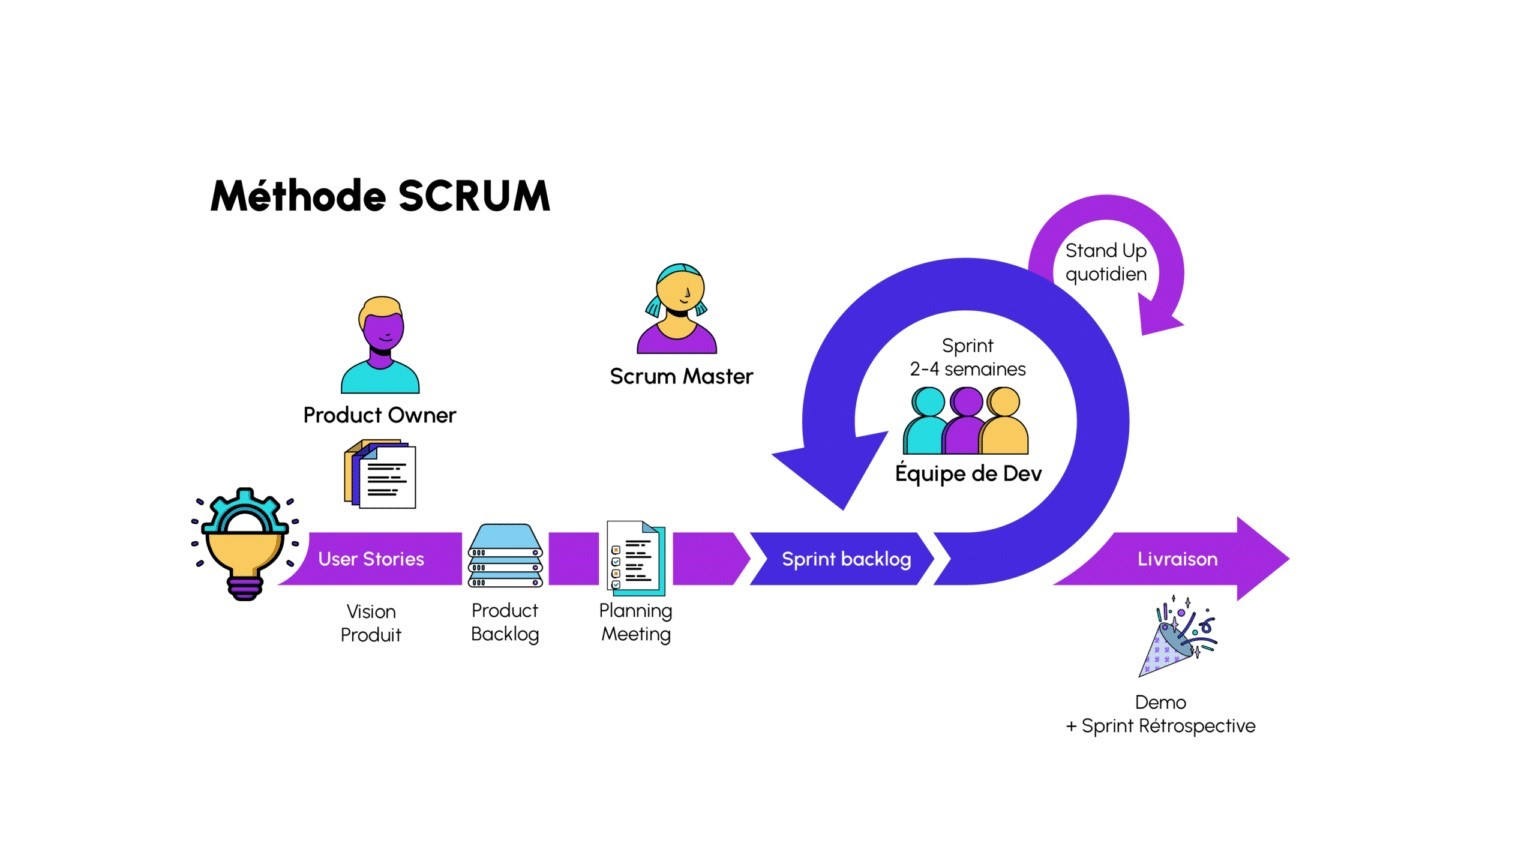
\includegraphics[width=0.9\linewidth]{projet/images/diagramme de sequance/images/methodeScrum.jpg}
    \caption{ Le processus de Scrum}
    \label{fig:image_centree}
\end{figure}


\addcontentsline{toc}{section}{Conclusion}
\section*{Conclusion}
Au cours de ce chapitre, nous avons présenté la société d’accueil « OMINET » ainsi que l’étude préalable, les méthodologies utilisées.
Dans le prochain chapitre, notre objectif est la planification du projet
